\chapter{Terrain}

% A few lines about heightmaps

The terrain itself is generated from a heightmap and is a continuation
of previous work, as already stated in the introduction. How a
heightmap is loaded from a texture and converted into geometry is
pretty straight forward, and thus won't be the focus in this
chapter. Instead we will focus on the lighting model and how it was
derived from the generel model presented in
\citebook{page~83}{RTR2}. We will talk about how we give the illusion
of more detailed geometry by implementing \emph{bump maps}, which
requires us to transform a bumped normal from \emph{tangent space} and
into \emph{world space}, where the lighting calculations are
done. Finally we will explain how \emph{texture arrays} where used to
cut back on \emph{texture unit} usage and texture lookups when
rendering.\\

% Geomorphing because it is in the vertex shader

However before we start, we must briefly touch upon the subject of
\emph{geomorphing} to understand part of what is going on in the vertex
shader.

% Geomorphing removes terrain popping

The heightmap uses cluster-based Continuous Level of Detail to
minimize vertex processing overhead. An example can be seen in
\reffig{fig:tesselation} where a mound is rendered with three
different levels of detail, LOD. When changing level of detail, the
terrain will appear to suddenly deform, this is termed \emph{Vertex
  Popping}. Geomorphing, as presented by \citeabook{1936}, can be used
to remove this popping by gently morphing in the new vertices. The
technique is rather simple. Instead of letting a vertex pop into it's
actual position when changing LOD, the vertex is created on the line
between it's two visible neighbours and then morphed into its actual
position. Because our terrain is a heightmap, geomorphing only needs
to be done along the y-axis.

\begin{figure}
  \centering
  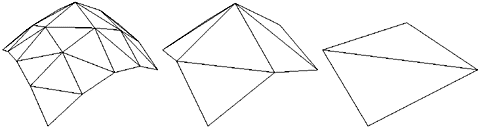
\includegraphics[width=5cm]{tesselation}
  \caption{A wireframe mound rendered with three different levels of
    detail. The new vertices introduced in higher levels of detail are
    the ones causing vertex popping.}
  \label{fig:tesselation}
\end{figure}

% We remove normal popping by using a normal map

Vertex popping has now been removed, but all other vertex attributes
must be morphed aswell to remove texture popping and normal
popping. Our heightmap texture coordinates are proportional to the
vertex xz-positions and will therefore not pop when changing LOD. But
the adding or removing of normals will cause popping in the
lighting. We could fix this by morphing the normals, but instead we've
used a \emph{normalmap} to store the normals in texture and look them
up in the fragment shader. This has the added benefit that we will
retain our light shading, even when the geometric detail is
reduced. The downside is that it forces us to use per pixel lighting,
since the normal is not available until the fragment shader.

We assume that the terrain is not rotated, scaled or translated, so
all our vertices and normals are given directly in world/model
space. This is done to simplify some of our calculations and save a
normal transformation in the fragment shader, but the theory can
easily be extended to transformed geometry.

\section{Lighting}

Because we are using shaders for rendering, we need to implement a
light model. The general lighting equation for one light
source\footnote{\citebook{page~83}{RTR2}} states

\begin{displaymath}
  \mathbf{i}_{tot} = \mathbf{a}_{glob} \otimes \mathbf{m}_{amb} +
  \mathbf{m}_{emi} + c_{spot}(\mathbf{i}_{amb} + d(\mathbf{i}_{diff} + \mathbf{i}_{spec}))
\end{displaymath}

Since the scene is set outside in a natural environment the only
lightsource is the sun, which is a directional light. This allows
several aspects of the lighting equation to be ignored. First of all
since there is only one lightsource in the scene, the global ambience
can be taken into account in the lightsource's ambience, removing that
expression from the equation.

\begin{displaymath}
  \mathbf{i}_{tot} = \mathbf{m}_{emi} + c_{spot}(\mathbf{i}_{amb} + d(\mathbf{i}_{diff} + \mathbf{i}_{spec}))
\end{displaymath}

Also because the lightsource is a directional light, the spotlight
factor, $c_{spot}$, and attenuation factor, $d$, can safely be
removed from the expression.

\begin{displaymath}
  \mathbf{i}_{tot} = \mathbf{m}_{emi} + \mathbf{i}_{amb} + \mathbf{i}_{diff} + \mathbf{i}_{spec}
\end{displaymath}

Lastly the emission factor is 0, since none of our surfaces emit
light, so we end up with

\begin{displaymath}
  \begin{array}{rl}
    \mathbf{i}_{tot} &= \mathbf{i}_{amb} + \mathbf{i}_{diff} +
    \mathbf{i}_{spec}\\
    &= \mathbf{m}_{amb} \otimes \mathbf{s}_{amb} + (\mathbf{n} \cdot
    \mathbf{l}) \mathbf{m}_{diff} \otimes \mathbf{s}_{diff} +
    (\mathbf{v} \cdot \mathbf{r})^{m_{shi}} \mathbf{m}_{spec} \otimes
    \mathbf{s}_{spec} 
  \end{array}
\end{displaymath}

where the following three formulas for ambient, diffuse and specular
lighting where used.

\begin{displaymath}
  \begin{array}{c}
    \mathbf{i}_{amb} = \mathbf{m}_{amb} \otimes \mathbf{s}_{amb} \\
    \mathbf{i}_{diff} = (\mathbf{n} \cdot \mathbf{l}) \mathbf{m}_{diff} \otimes \mathbf{s}_{diff} \\
    \mathbf{i}_{spec} = (\mathbf{v} \cdot \mathbf{r})^{m_{shi}} \mathbf{m}_{spec} \otimes \mathbf{s}_{spec} 
  \end{array}
\end{displaymath}

where $\mathbf{n}$ is the surface normal, $\mathbf{l}$ is the
direction of the light, $\mathbf{v}$ is the vector pointing to the
camera from the surface point and $\mathbf{r}$ is the reflection of the
light around the normal. All the vectors are assummed to be normalized
and can be seen on \reffig{fig:lightVectors}.

\begin{figure}
  \centering
  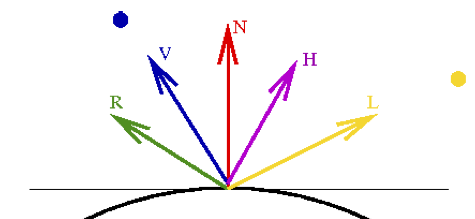
\includegraphics[width=5cm]{lightVectors}
  \caption{The vectors used in lighting calculations}
  \label{fig:lightVectors}
\end{figure}

\begin{figure}
  \centering
  \subfloat[Ambient lighting.]{
    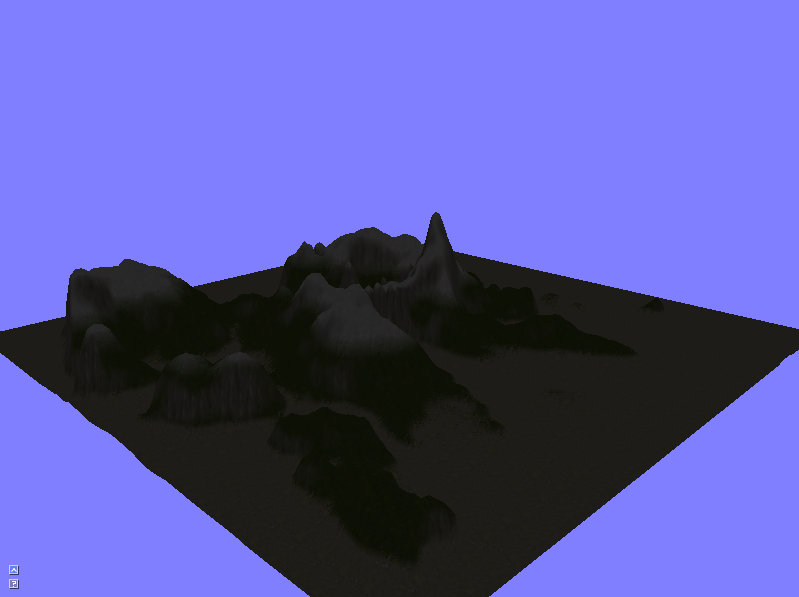
\includegraphics[width=6cm]{ambient}
  }
  \subfloat[Diffuse lighting.]{
    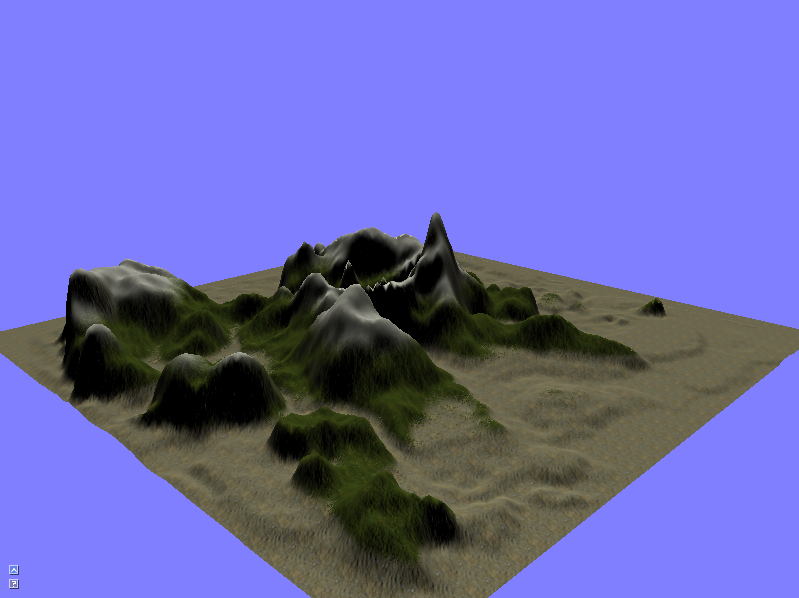
\includegraphics[width=6cm]{diffuse}
  }\\
  \subfloat[Specular lighting.]{
    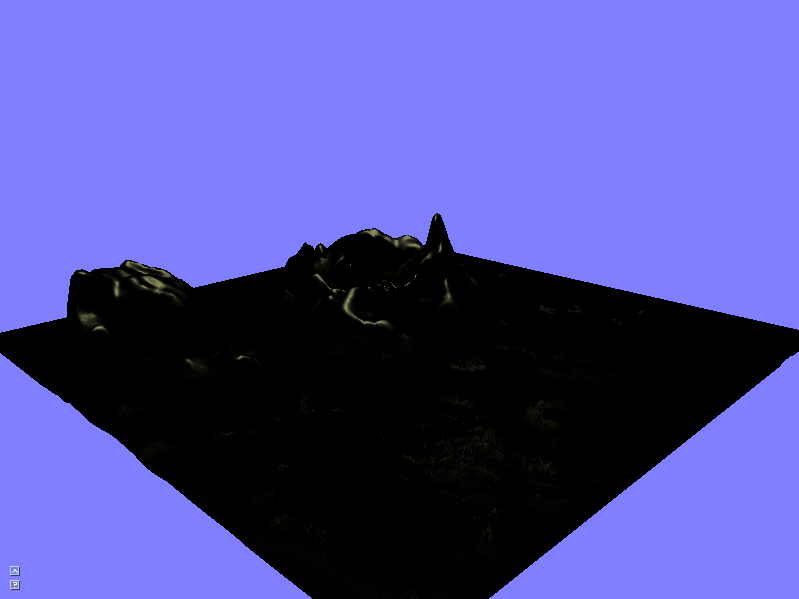
\includegraphics[width=6cm]{specular}
  }
  \subfloat[Combined lighting.]{
    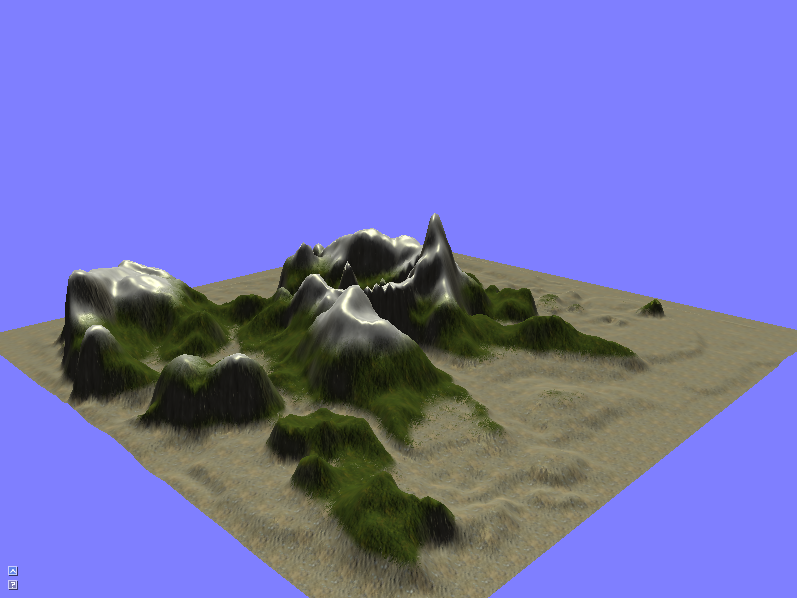
\includegraphics[width=6cm]{lightSum}
  }
  \caption{Images of the different light components making up the
    terrain lighting.}
  \label{fig:lightComponents}
\end{figure}


The contribution of each factor to the final image can be seen in
\reffig{fig:lightComponents}.

Now if we restrict our material to only specify one color and a
specular intensity instead of a seperat color for ambient, diffuse and
specular, we can reduce the equation to

\begin{displaymath}
  \begin{array}{rl}
    \mathbf{i}_{tot} &= \mathbf{m}_{color} \otimes \mathbf{s}_{amb} + (\mathbf{n} \cdot
    \mathbf{l}) \mathbf{m}_{color} \otimes \mathbf{s}_{diff} +
    (\mathbf{v} \cdot \mathbf{r})^{m_{shi}} \mathbf{m}_{color} \otimes
    \mathbf{s}_{spec} \\
    &= \mathbf{m}_{color} \otimes (\mathbf{s}_{amb} + (\mathbf{n} \cdot
    \mathbf{l}) \mathbf{s}_{diff} + m_{intensity} (\mathbf{v} \cdot
    \mathbf{r})^{m_{shi}} \mathbf{s}_{spec}) \\
  \end{array}
\end{displaymath}

This restriction is more physically correct, in the sense that only
the color of the material is now used with respect to the different
light components, but is also more restrictive to artists.\\

In the above formulas the specular lighting has been given by the
\emph{Phong lighting equation}\footnote{\citebook{page~76}{RTR2}},
$\mathbf{i}_{spec} = (\mathbf{v} \cdot \mathbf{r})^{m_{shi}}
\mathbf{m}_{spec} \otimes \mathbf{s}_{spec}$, where $\mathbf{m}_{spec}
= \mathbf{m}_{color}$ and $\mathbf{r} = 2 (\mathbf{n} \cdot
\ \mathbf{l}) - \mathbf{l}$.

A faster approximation was proposed by
Blinn\footnote{\citebook{page~77}{RTR2}}. Instead of basing the
specular highlight on the angle between the view direction and
reflection vector, he proposed to base it on the angle between the
normal and the halfvector, a vector halfway between the view- and
light direction given by $\mathbf{h} = (\mathbf{l} + \mathbf{v}) /
\|\mathbf{l} + \mathbf{v}\|$. An approximate relationship between the
two is given in \citebook{page~77}{RTR2} as

\begin{displaymath}
  (\mathbf{r} \cdot \mathbf{v})^{m_{shi}} \approx (\mathbf{n} \cdot \mathbf{h})^{4m_{shi}} 
\end{displaymath}

Both specular light models have been implemented in the terrain
fragment shader and the results can be seen in \reffig{fig:specularLight}

\begin{figure}
  \centering
  \subfloat[Phong specular lighting]{
    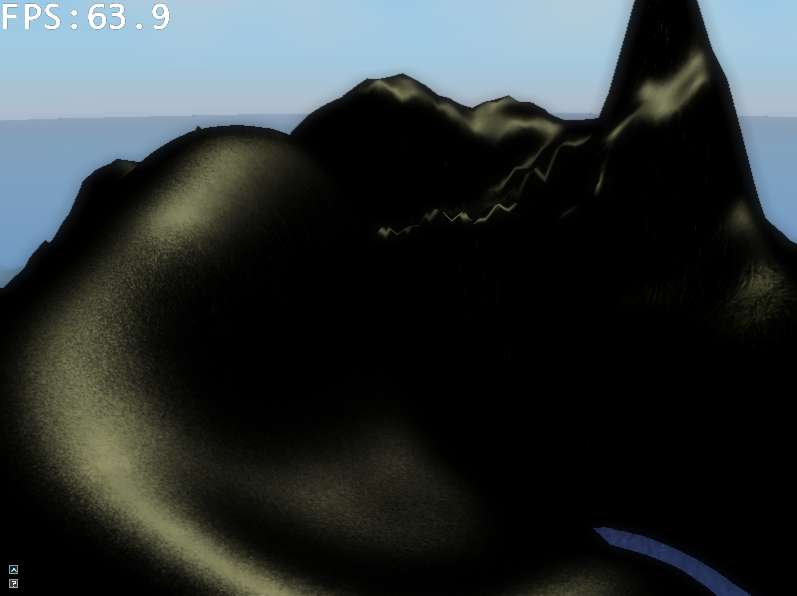
\includegraphics[width=5cm]{phongSpec}
  }
  \subfloat[Phong specular lighting]{
    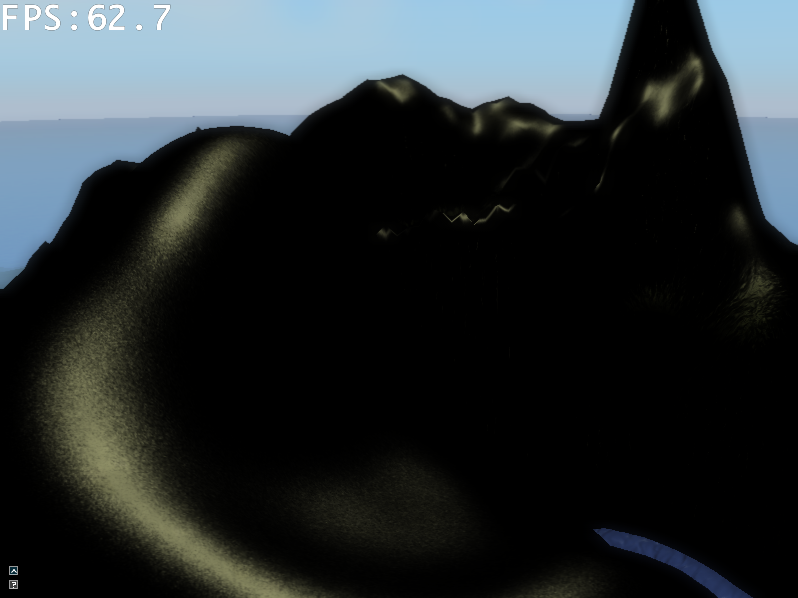
\includegraphics[width=5cm]{blinnSpec}
  }
  \caption{A comparison of Phong specular lighting and Blinn specular lighting.}
  \label{fig:specularLight}
\end{figure}

Since Blinn yields little to no framerate increase, we use Phong
specular lighting as the default, as it gives a more pleasing result.

The GLSL code for lighting with Phong specular light can be seen in
\reflst{lst:phongLighting}.

\begin{listing}
\centering
\begin{cppcode}
vec3 phongLighting(in vec3 text, in vec3 normal, in vec2 specProp){
  // Calculate diffuse
  float ndotl = dot(lightDir, normal);
  float diffuse = clamp(ndotl, 0.0, 1.0);
  
  // Calculate specular
  vec3 vRef = normalize(reflect(-lightDir, normal));
  float stemp = clamp(dot(normalize(eyeDir), vRef), 0.0, 1.0);
  float specular = specProp.x * pow(stemp, specProp.y);
  
  return text * (gl_LightSource[0].ambient.rgb + 
                 gl_LightSource[0].diffuse.rgb * diffuse + 
                 gl_LightSource[0].specular.rgb * specular);
}
\end{cppcode}
\caption{A GLSL function calculating lighting given a color, normal
  and specular intensity. The view/eye-and light direction are
  uniforms.}
\label{lst:phongLighting}
\end{listing}


\section{Bump mapping}

With the terrain shaded by the sun, it is time to improve on the detail
of the lighting by adding `bumps' to the surface, or more precisely
manipulating the normal to create a bumpy feel. This is done by
storing the normals of a surface in a normalmap texture, then instead of using
the interpolated geometric normal for light calculations, we transform
the texture normal into tangent space and use that for lighting.

In order to do this the interpolated normal, tangent and bitangent are
used as the axes of a tangent space coordinate system. Since we are
using the y-axis as up, the normal will be our y-axis in the tangent
space coordinate system. The tangent and bitangent are normalized
vectors perpendicular to the normal and lie along the normalmaps
texture coordinate axes. Calculating them normally is done as a
preprocessing step and they are stored as vertex attributes, or in our
case a tangent- and bitangentmap. However due to the heightmap being a
2D array of vertices with texture coordinates proportinal to the x-
and z-coordinates, we can calculate the tangents directly in the
shader. This saves us two texture lookup and the need to bind
additional textures.

Since our texture coordinates are axis-aligned, the tangent will lie
in the xy-plane and the bitangent is placed in the yz-plane. Below we
will show how to calculate the tangent, but the same principle can be
applied to calculate the bitangent.

The interpolated normal is our approximation of a vector perpendicular
to the terrain surface. It can therefore also be used to approximate
vectors along that surface, specifically the tangent along the
xy-plane. This is done by taking the cross product between the normal,
$n$, and the unit vector along the z-axis, $z_i = (0,0,1)$, which will
ensure that the tangent is both perpendicular to the normal, ie.
lying in the plane, and perpendicular to the z-axis, which places it
in the xy-plane. The calculations for the direction of the tangent are

\begin{displaymath}
  \begin{array}{rl}
  n \times z_i &= (n_x, n_y, n_z) \times (0,0,1)\\
  &= (n_y 1 - n_z 0, n_z 0 - n_x 1, n_1 0 - n_2 0) \\
  &= (n_y, - n_x, 0) \\
  \end{array}
\end{displaymath}

All that is left is to normalize the vector to get the tangent.

The tangent, bitangent and normal now make up the basis vectors of the
tangent space coordinate-system and can be used to either transform
the direction of the light from global space to tangent space or
transform the bumped normal from tangent space to global space. For
this project the latter was chosen to easier incorperate the shaders
into a deferred lighting pipeline in the future.

The GLSL code can be seen in \reflst{lst:bumpmapping}

\begin{listing}
\centering
\begin{cppcode}
  // Extract normal and calculate tangent and binormal
  vec3 normal = texture2D(normalMap, texCoord).xyz;
  vec3 tangent = normalize(vec3(normal.y, -normal.x, 0.0));
  vec3 bitangent = normalize(vec3(0.0, -normal.z, normal.y));
  mat3 tangentSpace = mat3(tangent, normal, bitangent);

  // Extract normals and transform them into tangent space
  vec3 bumpNormal = texture2DArray(normalTex, vec3(srcUV, layer)).xzy;
  bumpNormal = bumpNormal * 2.0 - 1.0; // move from [0; 1] to [-1; 1]
  bumpNormal = normalize(tangentSpace * bumpNormal);
\end{cppcode}
\caption{Calculating tangent space for a heightmap and rotating the normal in glsl.}
\label{lst:bumpmapping}
\end{listing}


\section{Texturing the terrain}

Several layers of color textures and normalmaps have been added to the
heightmap for a more diverse looking terrain. There is a sand layer, a
grass layer and a snow layer. Rocks have also been added on steep
slopes, but the focus is on layered texturing.

% No blending between layers

For our layered textures we chose to use the GL\_EXT\_texture\_array
extension, which allows us to create an array of textures that are
mipmapped individually. Unfortunately the texture array does not blend
across the different layers, so this has to be handled by the fragment
shader.

% We could have used a 3d texture instead but then we would loose
% mipmapping and we want our mipmapping!

An alternative would be placing all the layers in a three dimensional
texture, which could then blend between the different layers upon
texture lookup in the shader. The downside to this approach is that
using mipmapping on a three dimensional texture, will blend the
different layers together. In our case creating this creates a
brownish looking texture in the second mipmap level and downwards. The
only solution to this would be to disable mipmapping, which results in
a performance penalty and creates flickering textures.

In the end we opted for texture arrays over 3D textures and
implemented the blending ourselves. For each layer several parameters
can be chosen

\newcommand{\layerProp}[2]{\item \code{#1} - #2}
\begin{itemize}
  \layerProp{startHeight}{At what height the layer should start to
    blend in.}
  \layerProp{blending}{How many units of height it takes the layer to
    become completely opaque.}
  \layerProp{spec[i]}{The specular factor of the $i^th$ layer, where the
    x-component specifies a specular intensity scalar and the
    y-component is the shininess}
\end{itemize}

How much of the $i^th$ layer should be visible, $factor_i$, is then
trivially calculated by

\begin{displaymath}
  factor_i = (height - startHeight_i) / blending_i
\end{displaymath}

Since it does not make sense for a layer to be more than completely
transparent or opaque , ie. a factor of 0 or 1, we clamp the factor
between these values. The actual index of the layer to be used in the
texture array is then quite easy to calculate. We simply sum over all
the factors.

And example could be when layer 2 is completely opaque and layer 3 is
40\% visible. At that height layer 1 will also be completely
opaque. The layer height is then $1 + 1 + 0.4 = 2.4$, which means that
the base layer is 2 and that has be blended with 40\% of the 3'rd
layer.

When specifying the height or the terrain some randomness is added to
it from the normalmap. This is done to avoid smooth transitions
between the layers and give the terrain a more natural feel.


%%% Local Variables:
%%% mode: latex
%%% TeX-master: t
%%% TeX-PDF-mode: t
%%% End:
